% ------------------------------------------------------------------------------
%     前言区域
% ------------------------------------------------------------------------------
\documentclass{beamer}
\usepackage{ctex}
% \usepackage{CJK}
\usepackage{hyperref}
% \usepackage[T1]{fontenc}


% other packages
\usepackage{latexsym,amsmath,xcolor,multicol,booktabs,calligra}
\usepackage{graphicx,pstricks,listings,stackengine}
\usepackage{subfigure}
\usepackage{amsfonts}
\usepackage{amssymb}
% \usepackage{subcaption}

\usepackage[mathlines]{lineno}% Enable numbering of text and display math
%\usepackage{mathptmx}
\setmainfont{SimSun} % or another available font
% ------------------------------------------------------------------------------
%     标题页
% ------------------------------------------------------------------------------
\author{仝佳驹}
\title{Incremental Constrained Clustering by Minimal
Weighted Modification}
% \subtitle{}
% \institute{}
\date{2024-12-10}
\usepackage{uir}
%\logo{\includegraphics[width=0.5 cm]{Picture/uir.jpeg}} % 每一页添加logo

% defs
\def\cmd#1{\texttt{\color{red}\footnotesize $\backslash$#1}}
\def\env#1{\texttt{\color{blue}\footnotesize #1}}
\definecolor{deepblue}{rgb}{0,0,0.5}
\definecolor{deepred}{rgb}{0.6,0,0}
\definecolor{deepgreen}{rgb}{0,0.5,0}
\definecolor{halfgray}{gray}{0.55}

\lstset{
    basicstyle=\ttfamily\small,
    keywordstyle=\bfseries\color{deepblue},
    emphstyle=\ttfamily\color{deepred},    % Custom highlighting style
    stringstyle=\color{deepgreen},
    numbers=left,
    numberstyle=\small\color{halfgray},
    rulesepcolor=\color{red!20!green!20!blue!20},
    frame=shadowbox,
}

\graphicspath{{./Picture/}} % 图片所在位置

% ------------------------------------------------------------------------------
%     正文
% ------------------------------------------------------------------------------
\begin{document}

%\kaishu
%\rmfamily
\begin{frame}
    \titlepage
    %\begin{figure}[htpb]
    %    \begin{center}
    %        \includegraphics[width=0.2\linewidth]{Picture/uir.jpeg}
    %    \end{center}
    %\end{figure}
\end{frame}

% \begin{frame}
%     \tableofcontents[sectionstyle=show,subsectionstyle=show/shaded/hide,subsubsectionstyle=show/shaded/hide]
% \end{frame}

\section{Background}

\begin{frame}{Clustering}
\begin{itemize}
\item Clustering

给定数据集$X=\{x_i\}_{i=1}^n$,将数据集划分为若干个不相交的子集,每个子集称为一个簇。同一簇中的数据对象之间相似度较高,不同簇中的数据对象之间相似度较低。

一种无监督学习

\item Constraint Clustering

约束聚类旨在通过约束的形式找到满足某些性质的聚类结果。

例如:ML(Must-Link)约束,CL(Cannot-Link)约束。

将无监督学习转化为半监督学习。

\item Incremental Constraint Clustering

增量式约束聚类是指在已有的聚类结果上,通过添加约束,来调整原有的聚类结果。
\end{itemize}
\end{frame}

\begin{frame}{Human in the Loop}

在实践中需要领域专家的知识来指导聚类过程

困难:只基于数据给出约束。

简易:根据当前聚类结果提供反馈来改进聚类。
    
\begin{itemize}
\item Requests:
与人交互,因此每步的更新应够快。与前一步的结果相似。

\item Problems:如何整合约束信息,如何保持聚类结果的稳定性,如何处理相矛盾的约束。

\end{itemize}

\end{frame}


\section{Framework}

\begin{frame}{Incremental and Active Clustering Framework}


\begin{figure}[htpb]
    \begin{center}
        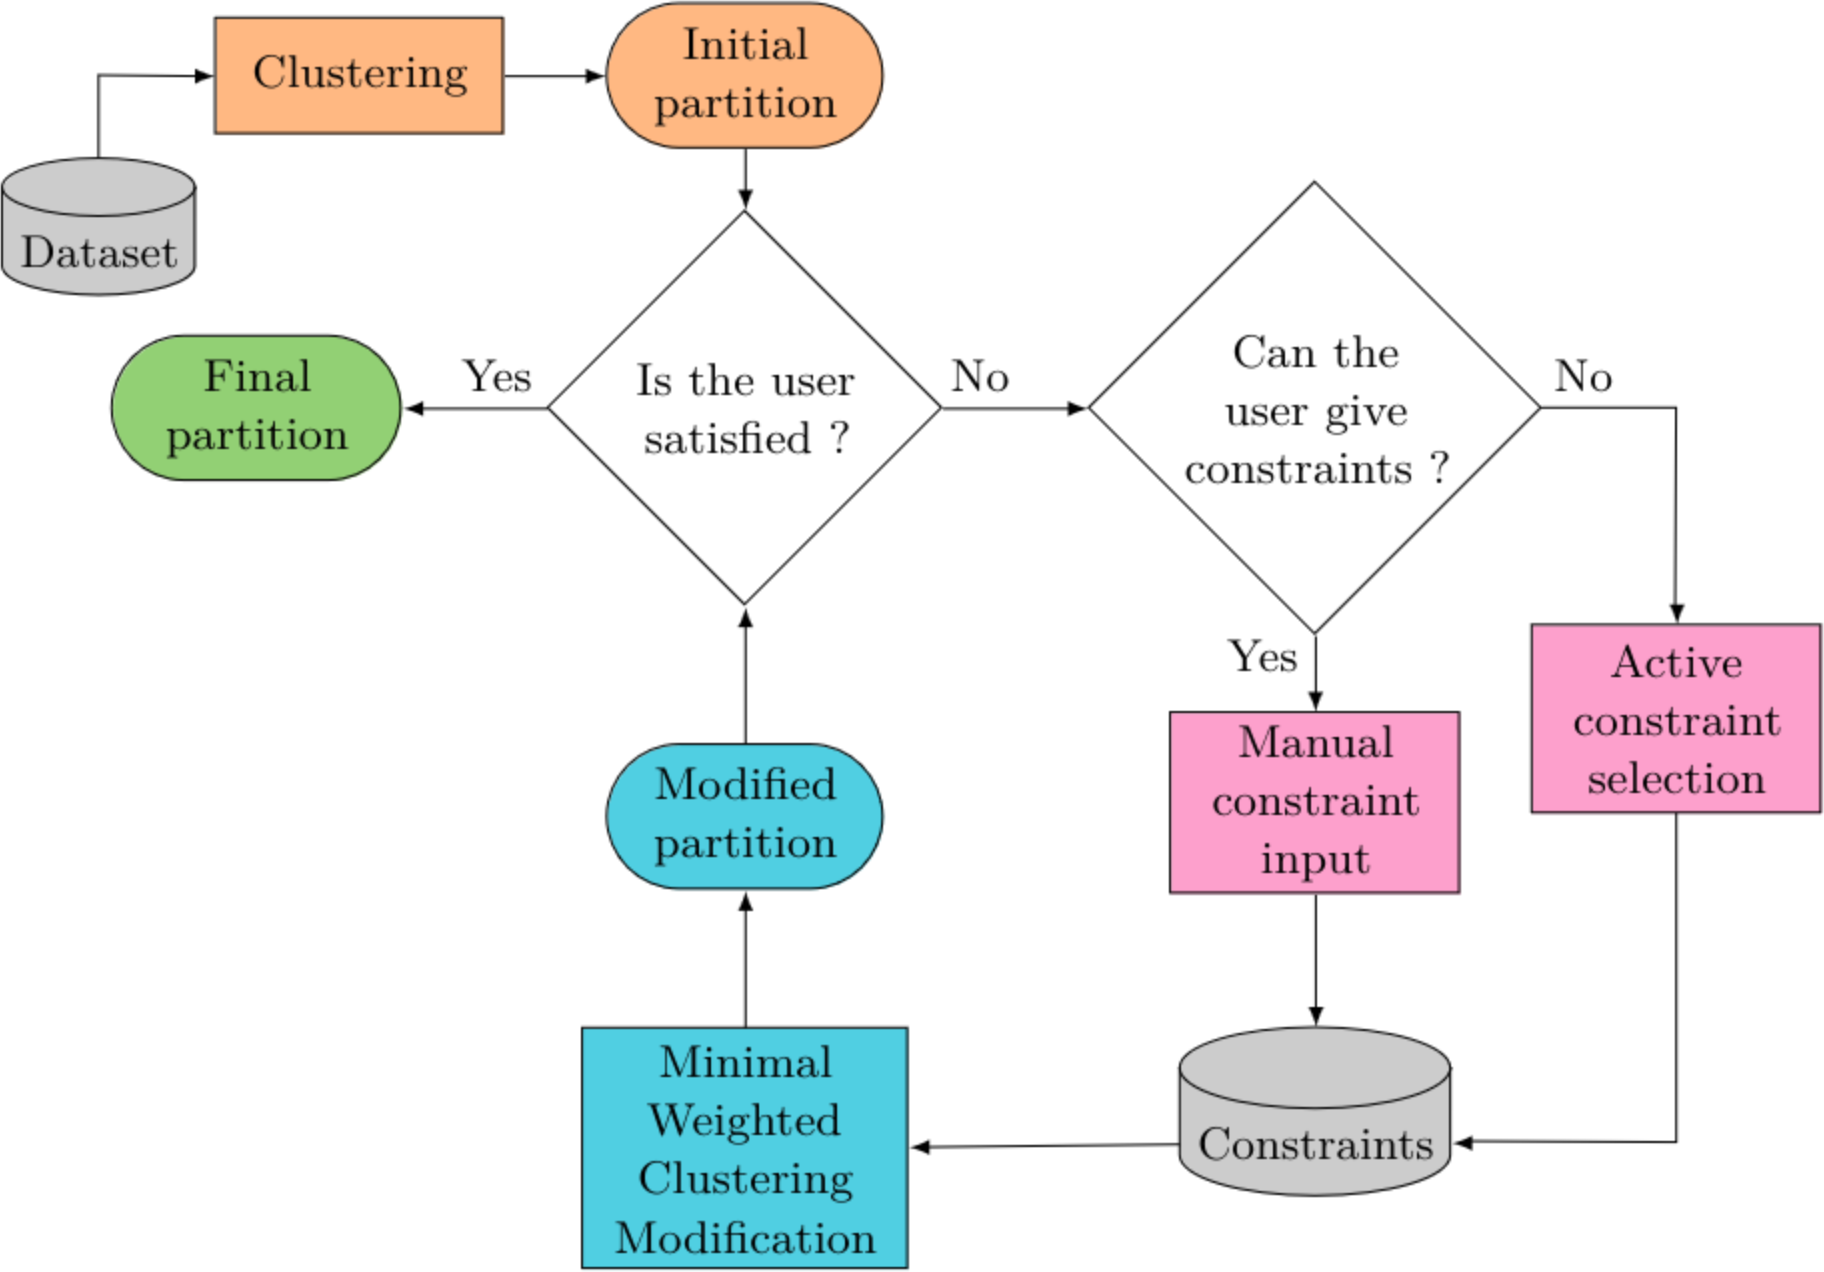
\includegraphics[width=0.8\linewidth]{./images/scheme.png}
    \end{center}
\end{figure}


\end{frame}

\begin{frame}{Mannual Constraints}
    \begin{columns}
        \begin{column}{0.3\textwidth}
            \begin{figure}[htpb]
                \begin{center}
                    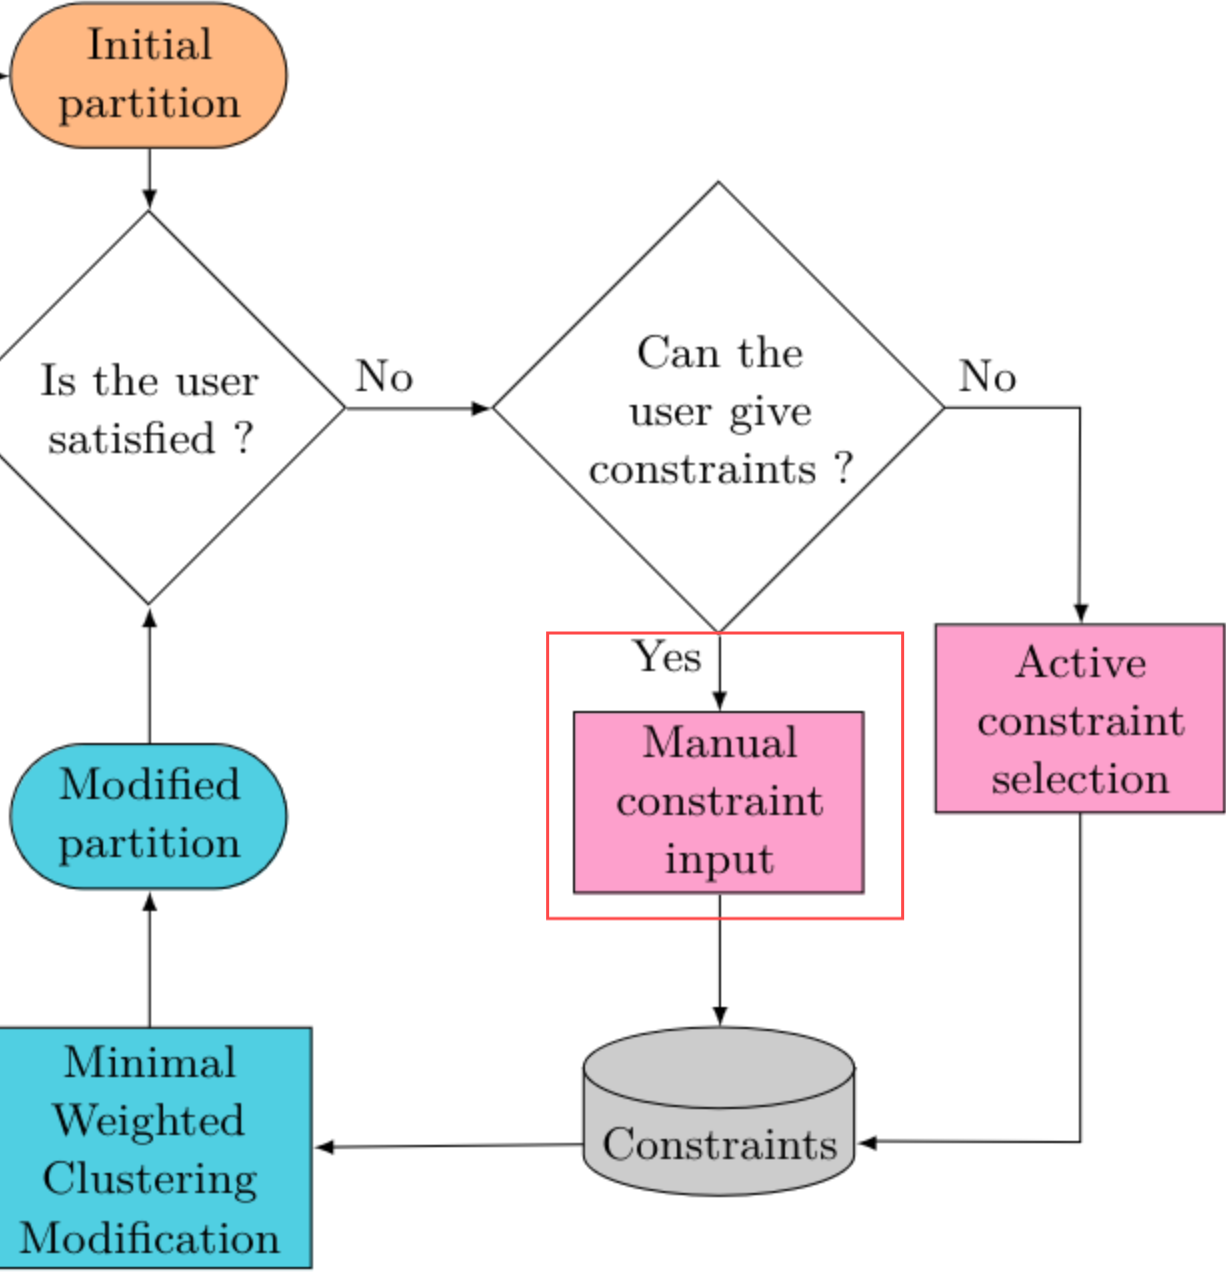
\includegraphics[width=\linewidth]{./images/constraint.png}
                \end{center}
            \end{figure}
        \end{column}     
        \begin{column}{0.6\textwidth}
            用户给出约束

            \begin{itemize}
                \item Must-Link\&Cannot-Link
                \item Triplets Constraints:$(x,p,n)$\\ x与p比n更相似。即$G_x=G_n\Rightarrow G_x=G_p$
                \item Span-limited Constraints:$S\subset X,C\subseteq [1,K]$\\
                S中的点只能在C中的簇中。
                \item a generic span-limited constraint:given $\gamma$\\
                S中的点最多在$\gamma$个簇中。
                \item \text{implicit constraint}:\\
                $P\Rightarrow Q$,P,Q为ML/CL的合取式
            \end{itemize}
        \end{column}
    \end{columns}


\end{frame}

\begin{frame}{Active Constraints Selection}
    
    \begin{columns}
        \begin{column}{0.5\textwidth}
            \begin{figure}[htpb]
                \begin{center}
                    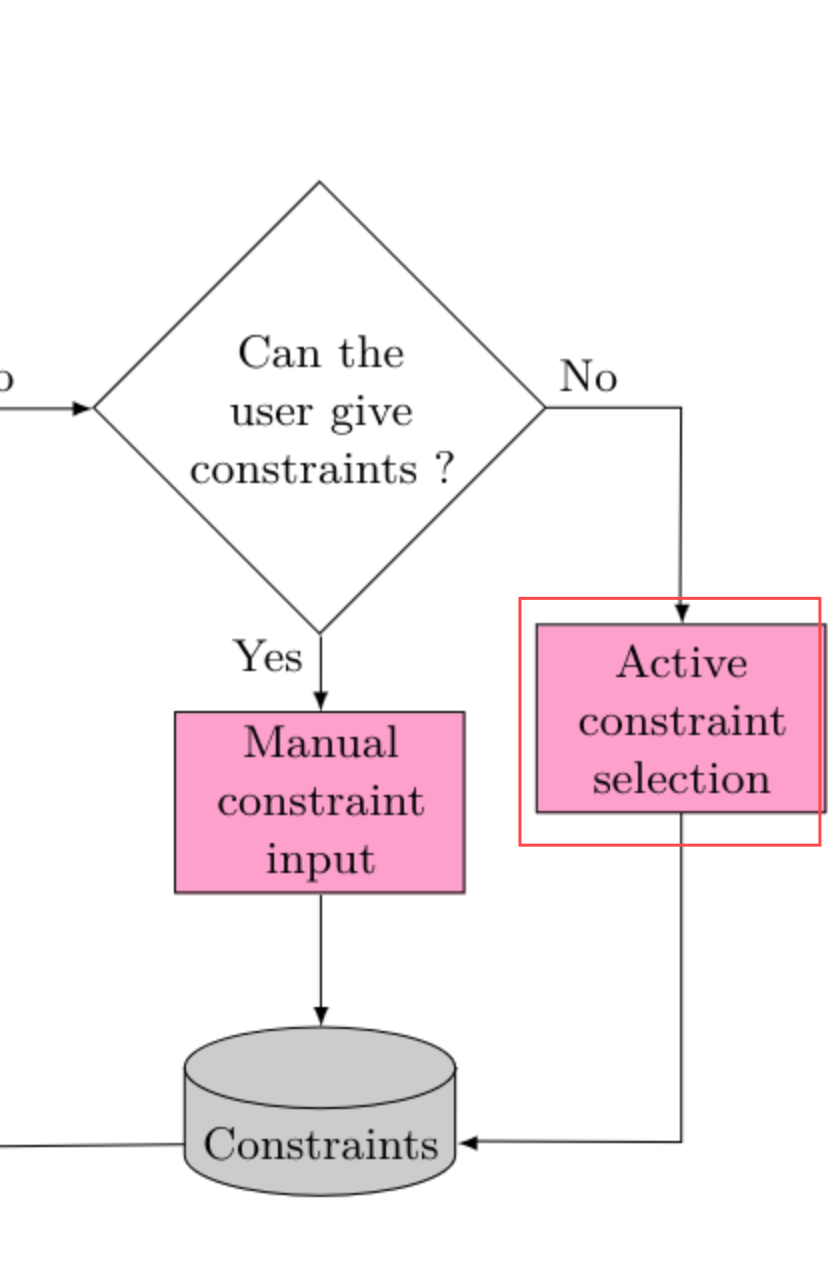
\includegraphics[width=0.8\linewidth]{./images/selection.png}
                \end{center}
            \end{figure}
        \end{column}     
        \begin{column}{0.48\textwidth}
            选择most informative的点,query它与其他数据间的约束。

            具体方法:NPU(Neighborhood-based Pairwise Uncertainty)



        \end{column}
    \end{columns}
\end{frame}

\begin{frame}{Modication}
    \begin{columns}
        \begin{column}{0.5\textwidth}
            \begin{figure}[htpb]
                \begin{center}
                    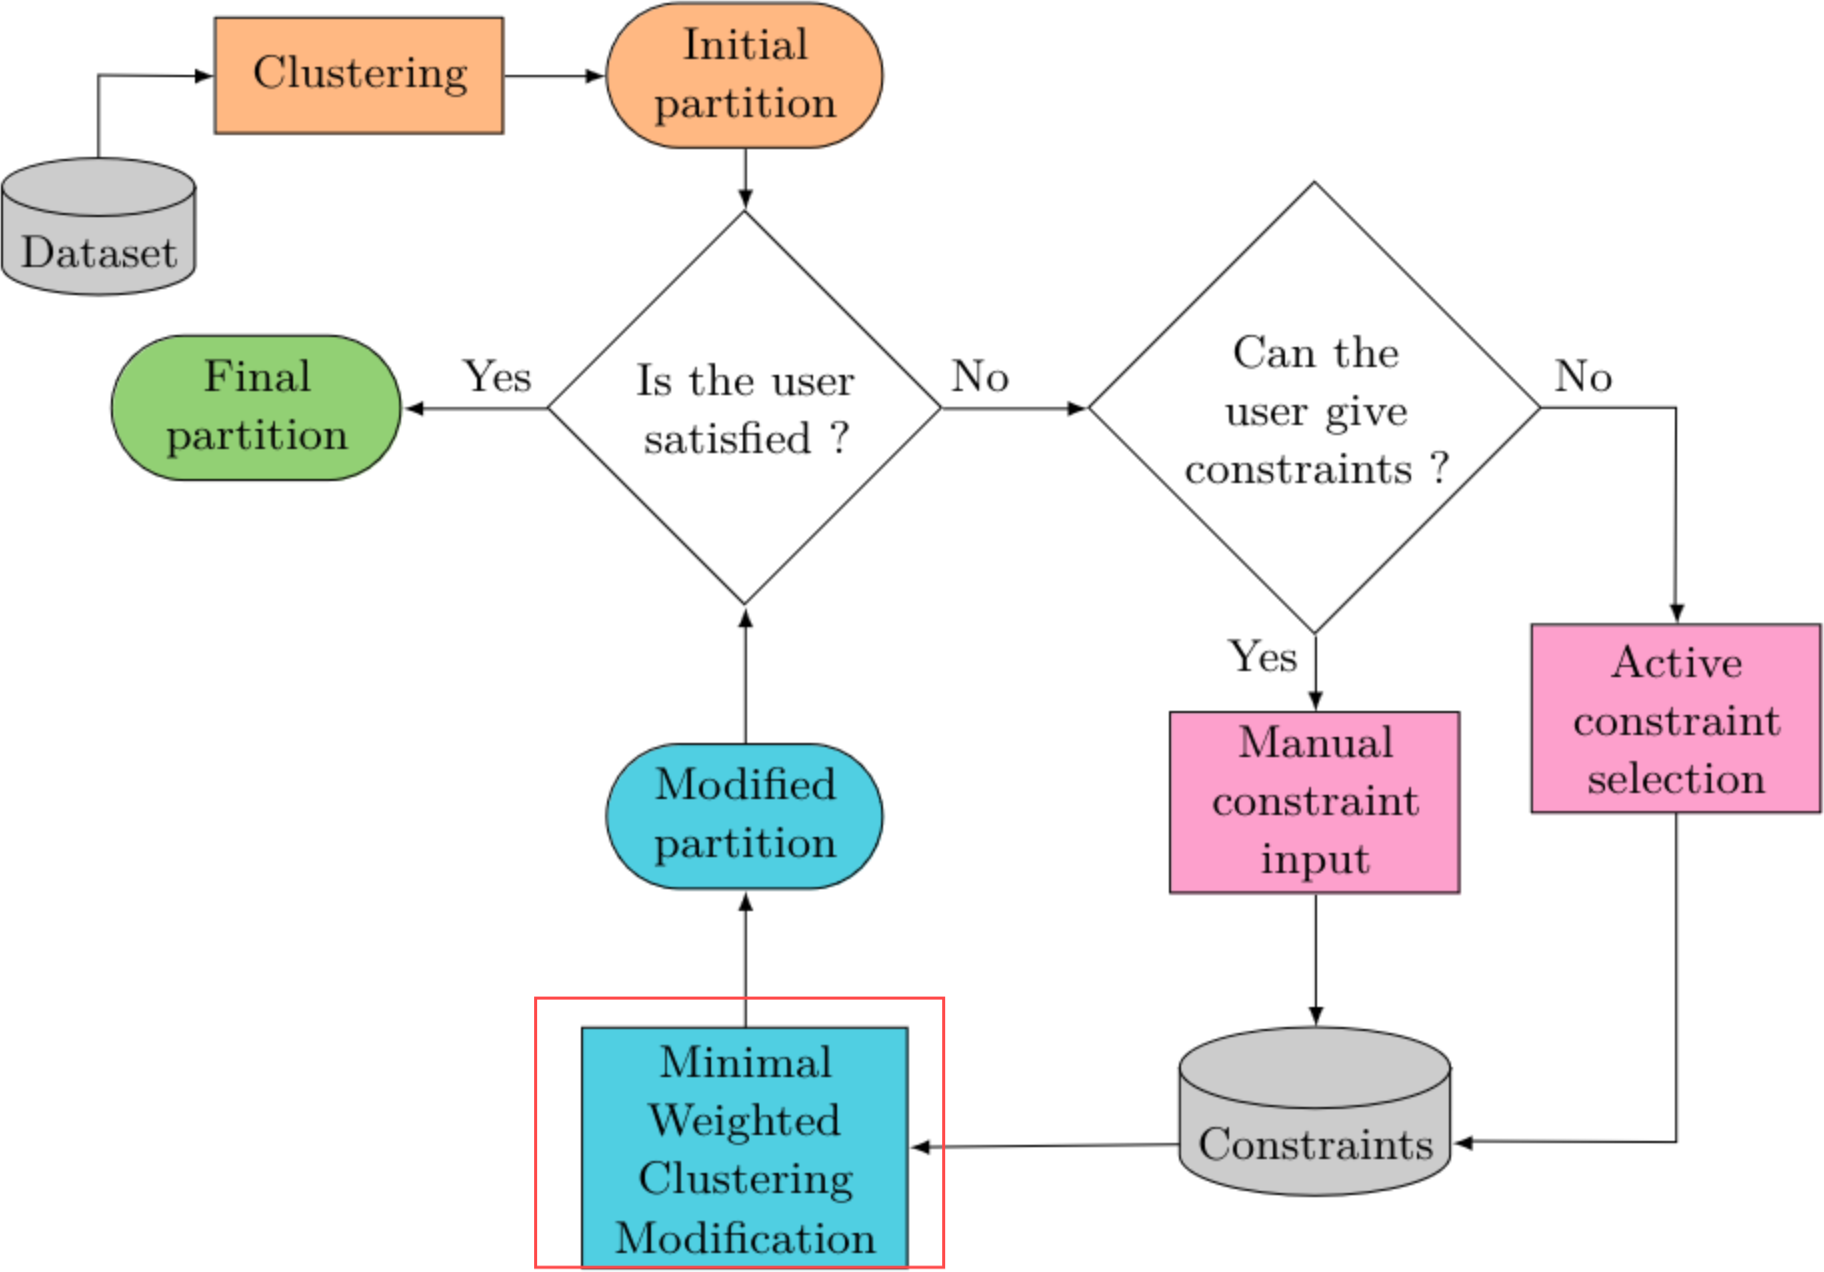
\includegraphics[width=0.8\linewidth]{./images/modify.png}
                \end{center}
            \end{figure}
        \end{column}     
        \begin{column}{0.48\textwidth}
            given partition $\mathcal{P}$,user constraints $\mathcal{C}$,...

            根据$\mathcal{C}$,对$\mathcal{P}$进行修改。
            
            $f$为度量partition间的差异的函数。

            $\mathcal{P}'=\arg\min f(\mathcal{P}',\mathcal{P})$
            
        \end{column}
    \end{columns}
    
\end{frame}

\section{Modification}

\begin{frame}{Minimal Weighted Clustering Modification(MWCM)}
    \begin{figure}
        \centering
        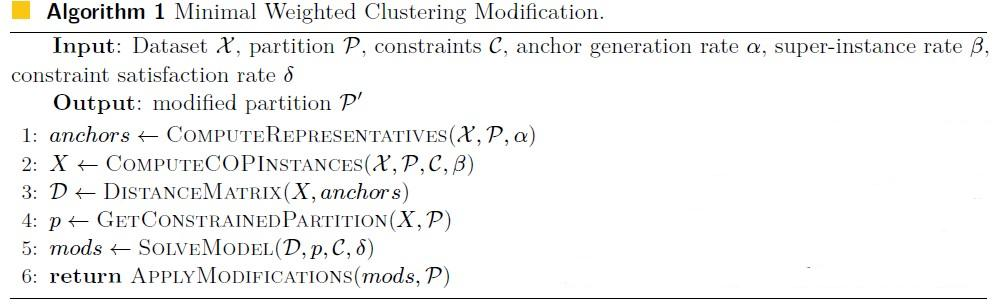
\includegraphics[width=0.8\linewidth]{./images/mwcm.jpg}
        \caption{MWCM}
        \label{fig:mwcm}
    \end{figure}    
\begin{enumerate}
    \item 计算$\mathcal{P}$的代表: anchors
    \item 计算$\mathcal{P}$的super instances(用于后续Constraint Optimization Problem)
    \item 创建距离矩阵$\mathcal{D}$(用于后续COP)
    \item 计算X的clustering $p$
    \item 根据$\mathcal{D},p,\mathcal{C}$求解X新的clustering $mods$
    \item 从$mods$得到新的partition $\mathcal{P}'$
\end{enumerate}


\end{frame}


\begin{frame}{Objective Function}
    \begin{itemize}
        \item naive objective function:
$$\arg\min\sum\limits_{i=1}^N \mathbb{I}(\mathcal{P}[i]\neq\mathcal{P}'[i])$$

\item take into account the structure of the clusters:
$$\arg\min\sum\limits_{i=1}^N \mathbb{I}(\mathcal{P}[i]\neq\mathcal{P}'[i])\mathcal{D}[i,\mathcal{P}'[i]]$$
$\mathcal{D}[i,c]$为i与cluster c的距离。

    \end{itemize}
    
\end{frame}


\begin{frame}{Anchors}
    \begin{itemize}
        \item $\mathcal{D}[i,c]=d(i,\mu_c)$ ,$\mu_c$ is cluster c's medoids.\\
        implicitly treat all clusters as spherical
        \begin{figure}
            \centering
            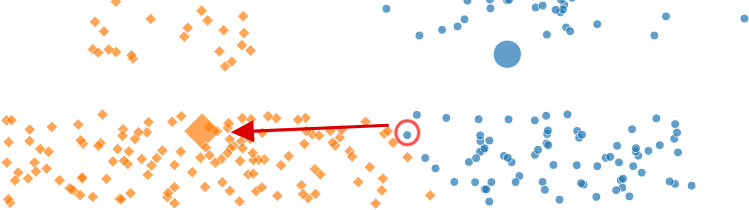
\includegraphics[width=0.8\linewidth]{./images/medoids.png}
        \end{figure}
        \item anchors: representative points of sub-clusters of a cluster.\\
        $\mathcal{D}[i,c]$ represents the distance of instance i to its closest anchor belonging to cluster c
    \end{itemize}




\end{frame}


\begin{frame}{Anchors}
    \begin{columns}

        \begin{column}{0.48\textwidth}
            \begin{itemize}
                \item How to get sub-clusters of a cluster?$\Leftarrow$ \text{sigle-link hierarchical clustering }\\
                适合发现任意形状的簇
                \begin{figure}
                    \centering
                    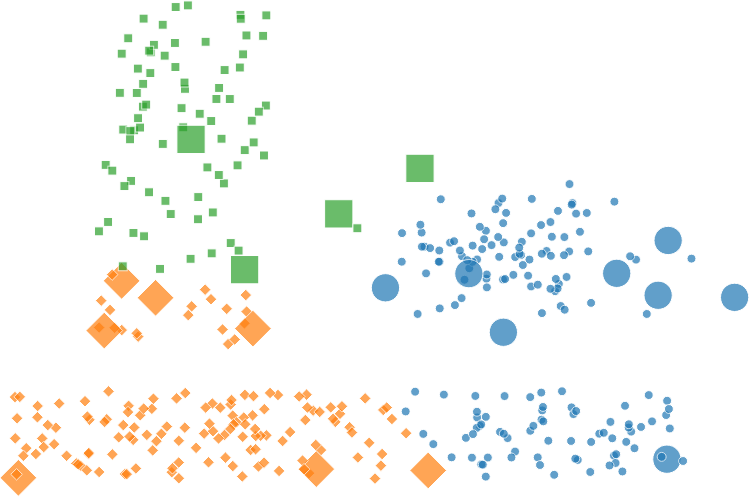
\includegraphics[width=0.8\linewidth]{./images/anchors.png}
                \end{figure}
                \item $\alpha$:proportion of anchors per cluster.
            \end{itemize}

        \end{column}
        \begin{column}{0.4\textwidth}
            \begin{figure}[htpb]
                \begin{center}
                    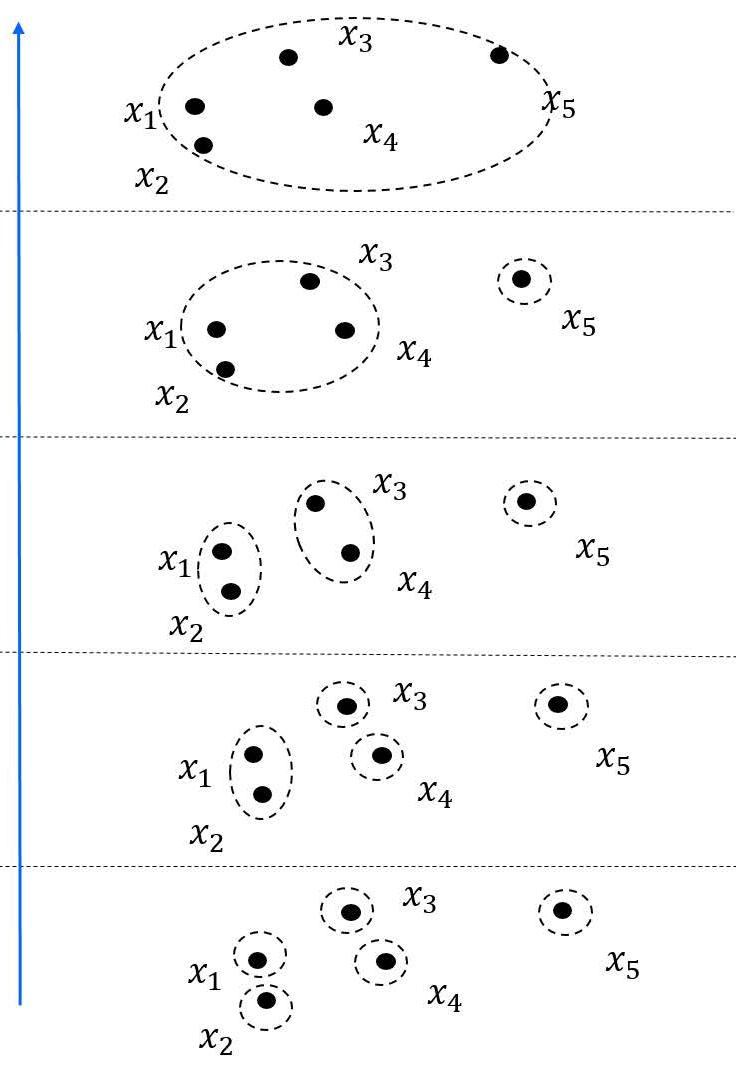
\includegraphics[width=\linewidth]{./images/cluster.jpg}
                \end{center}
            \end{figure}
        \end{column}             
    \end{columns}
    
\end{frame}



\begin{frame}{Super Instances}
\begin{figure}
    \centering
    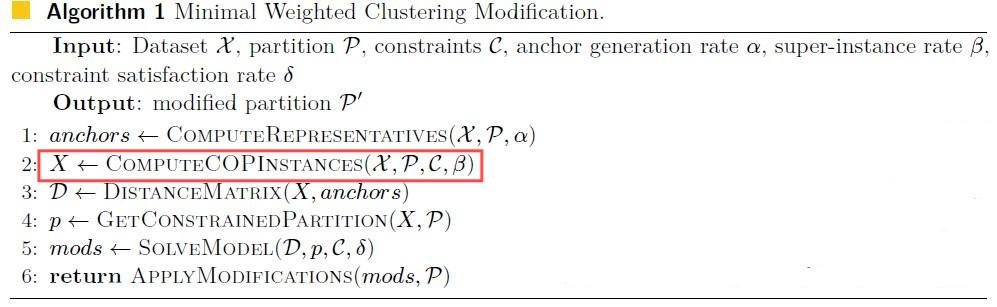
\includegraphics[width=0.8\linewidth]{./images/super.jpg}
\end{figure} 
\begin{itemize}
    \item 在实践中,专家只能对少数数据给出约束反馈,相对于数据集甚至可以忽略。
    \item 假设专家想要调整的是选择的点周围的区域内所有的点,而不是单单是点本身。
    \item super-instances:virtual instances grouping several real data points
    \item 推广被约束点的约束到其周围的点。
\end{itemize}




\end{frame}

\begin{frame}
    \frametitle{Super Instances}

    \begin{itemize}
        \item How to get super instances?\\
        complete-link hierarchical clustering
        \item user constraints$\rightarrow$ super instances constraints\\
        潜在的约束冲突风险?\\
        确保每个super instance只有不多于一个被约束的数据点。
    \end{itemize}
    

\end{frame}

\begin{frame}{Super Instances}

    \begin{figure}
        \centering
        \subfigure[previous partition]{
            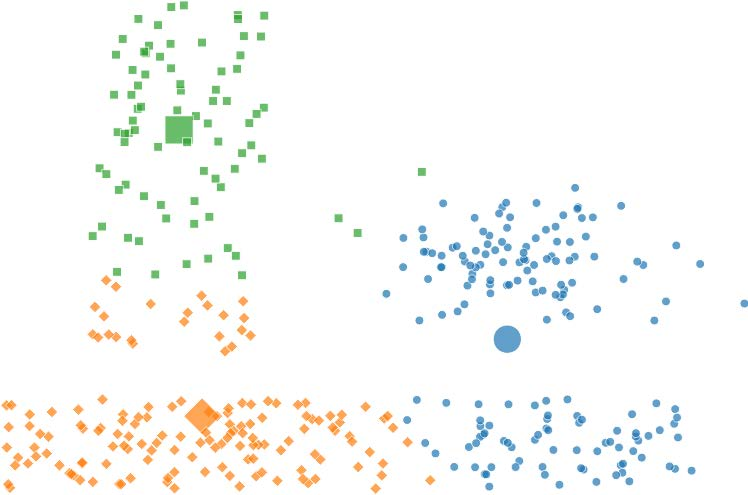
\includegraphics[width=0.45\linewidth]{./images/super1.jpg}
        }
        \subfigure[complete-link clustering]{
            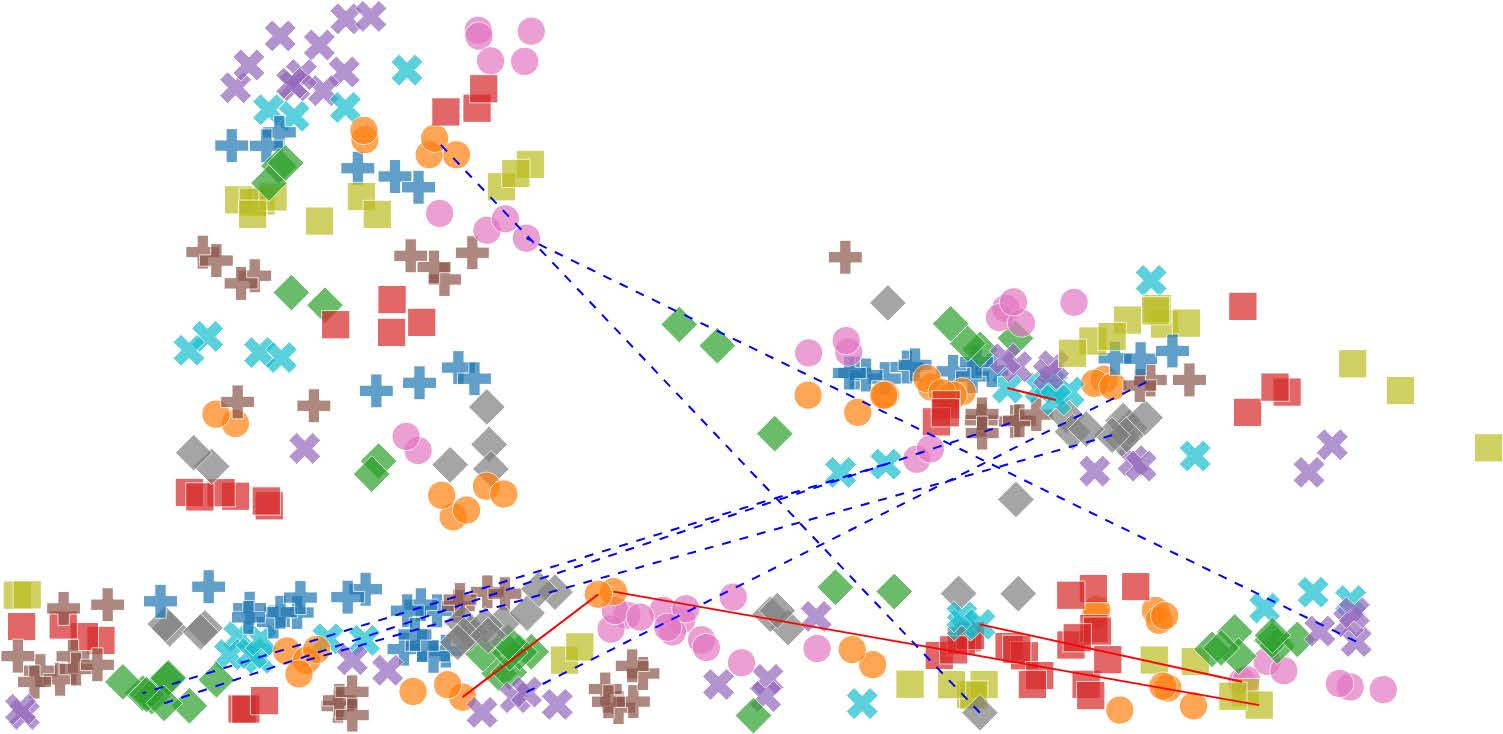
\includegraphics[width=0.45\linewidth]{./images/super2.jpg}
        }
        \subfigure[super instances]{
            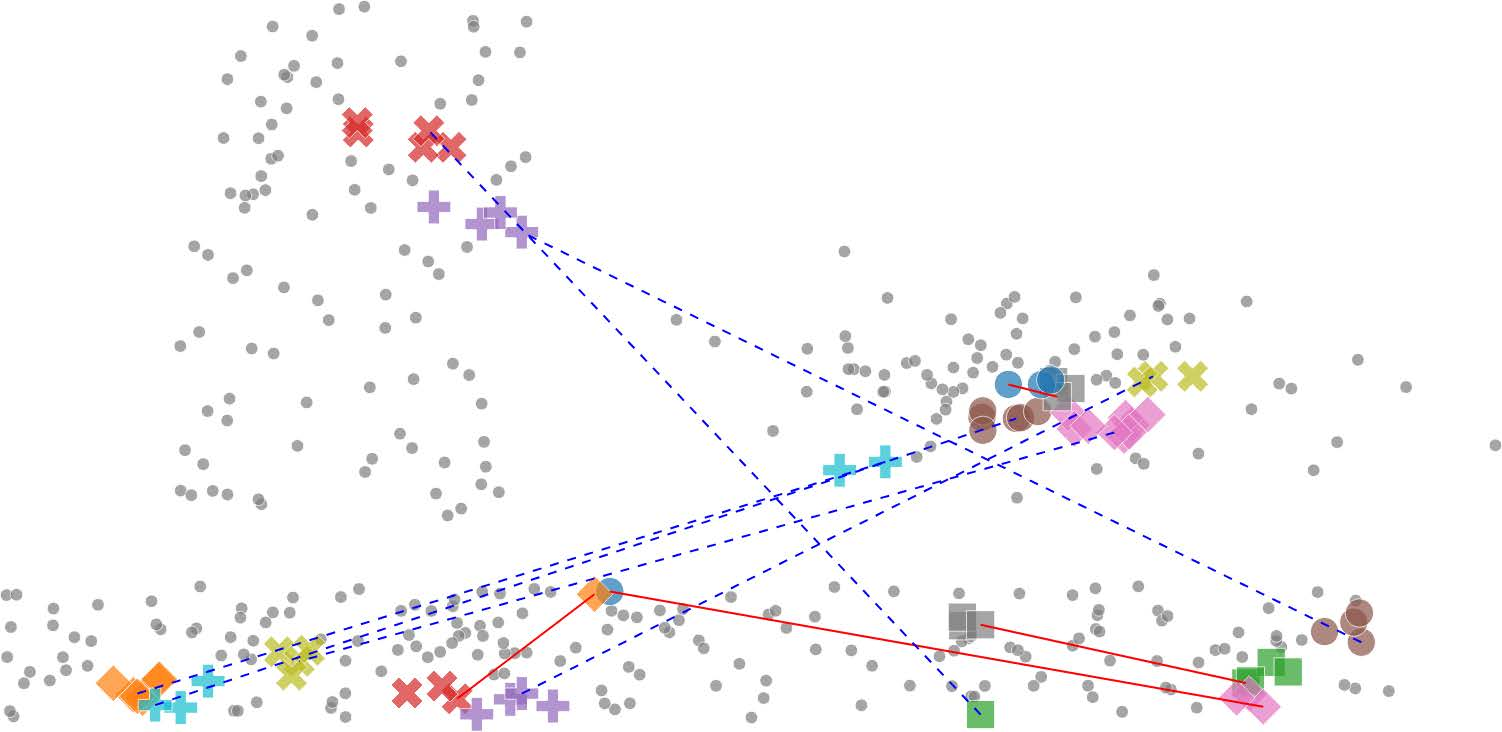
\includegraphics[width=0.45\linewidth]{./images/super3.jpg}
        }
    \end{figure}
    
\end{frame}

\begin{frame}{Apply Modification}
    \begin{figure}
        \centering
        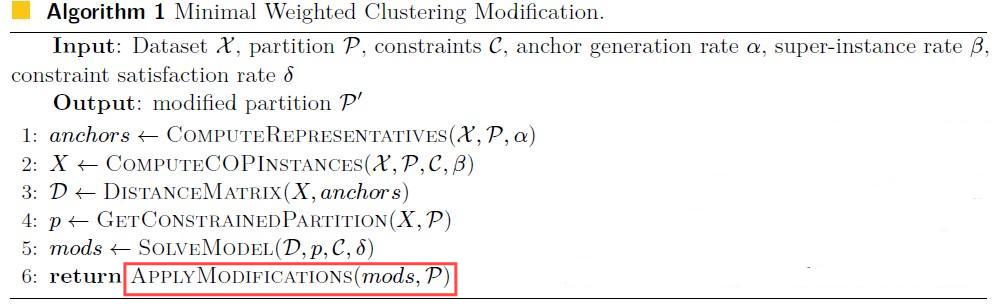
\includegraphics[width=\textwidth]{./images/apply.jpg}
    \end{figure}
    \begin{figure}
        \centering
        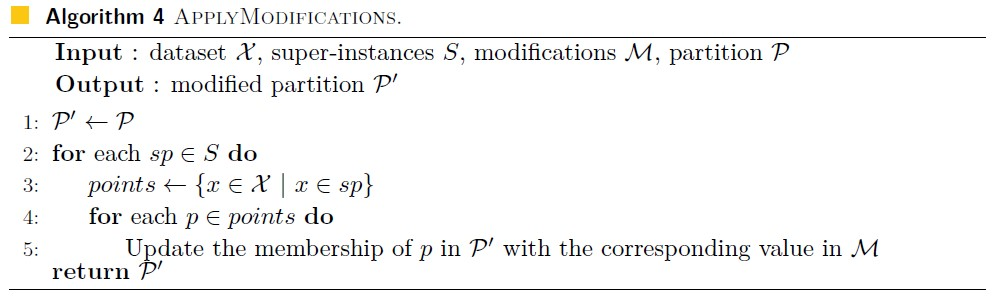
\includegraphics[width=\textwidth]{./images/modification.jpg}
    \end{figure}
\end{frame}


\section{Constraint Optimization}

\begin{frame}{Variables}
\begin{itemize}
    \item 
variables:for each $ i\in X$,$G_i$ with domain $[1,K]$

$G_i=c$ means instance i  to cluster c in new partition $\mathcal{P}'$
\item objective function:
$$\arg\min\sum\limits_{i\in X} \mathbb{I}(G_i\neq\mathcal{P}[i])\mathcal{D}[i,G_i]$$

\end{itemize}

\end{frame}

\begin{frame}{Handling Conflicting Constraints}
\begin{itemize}
    \item 可以设置$G_i$的domain为$[1,K'],K'>K$,允许新的簇的产生。\\
    防止instance从优化上被分到新的簇:\\
    set $\mathcal{D}[i,k'],k\in [K+1,K']$ greater
    \item Relaxing constraints:\\
    $\sum\limits_{c\in\mathcal{C}}S_c \overset{>}{\underset{<}{=}} \delta |\mathcal{C}|$, where $S_c=1$ iff c is satisfied\\
\end{itemize}


\end{frame}

\section{Active Constraint Selection}
\begin{frame}{Active Constraints Selection}
    \begin{itemize}
        \item Neighborhoods $\mathcal{N}$:groups
        of instances whose cluster assignment is certain
        \item 
    to construct $\mathcal{N}$,iteratively do:
    \begin{itemize}
        \item select the most informative instance $x^*$
        \item query the relationship between $x^*$ N in $\mathcal{N}$,add ML/CL constraints
        \item if no ML added,create a new neighborhood with $x^*$
    \end{itemize}
    \begin{figure}
        \centering
        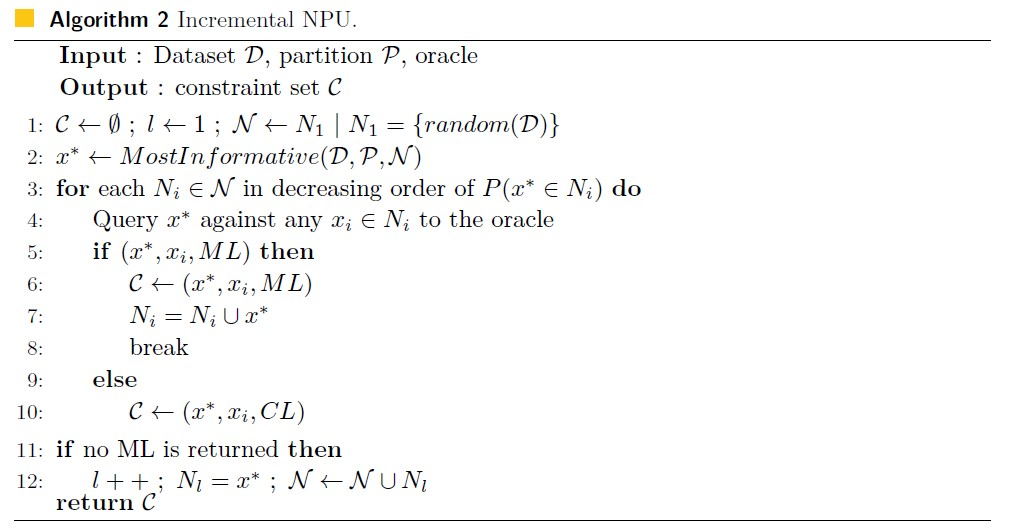
\includegraphics[width=0.6\linewidth]{./images/npu.jpg}
    \end{figure}
\end{itemize}
\end{frame}

\begin{frame}{Active Constraints Selection}
    \begin{itemize}
        \item Neighborhood-based Pairwise Uncertainty(NPU)
        \begin{itemize}
        \item $H(\mathcal{N}|x)$:entropy measure of
        the uncertainty to assign x to a neighborhood in $\mathcal{N}$
        \item $\mathbb{E}(q(x))$:expected number of queries to discover its neighborhood
        \item informativeness:$\frac{H(\mathcal{N}|x)}{\mathbb{E}(q(x))}$
        \end{itemize}
    \end{itemize}
    \begin{figure}
        \centering
        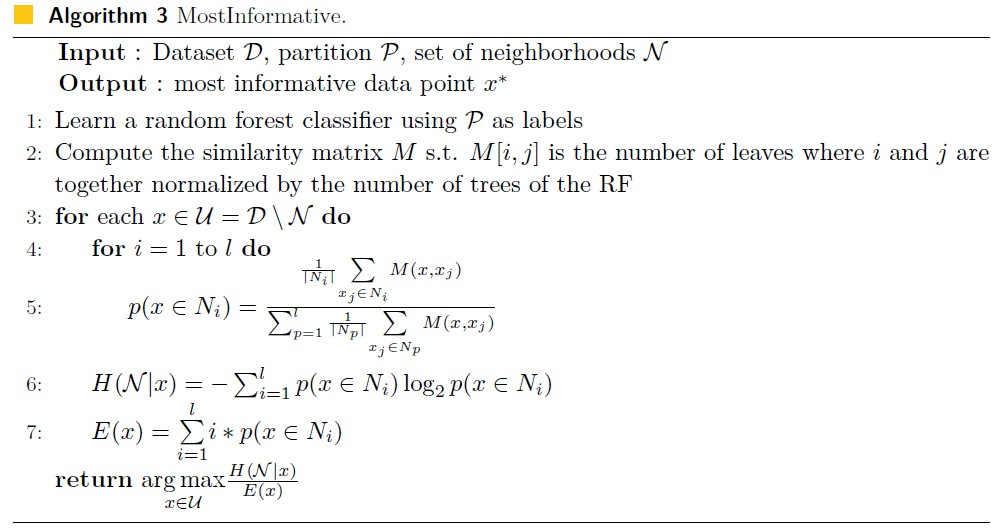
\includegraphics[width=0.6\linewidth]{./images/inform.jpg}
    \end{figure}
\end{frame}


\section{Experiments}
\begin{frame}{Methodology}
    \begin{itemize}
        \item Evaluating single partition:
        \begin{itemize}
            \item Functions measuring similarity between partitions:ARI,AMI,FMI...
            $$ARI(\mathcal{P}_1,\mathcal{P}_2)=\cdots$$
        \end{itemize}
        \item Evaluating all partitions:
        \\ area under the budget curve(AUBC)
        \\ two types:
        \begin{itemize}
            \item $AUBC_\text{quality}$ when compare partitions with ground truth
            \item $AUBC_\text{similarity}$ when compare partitions with previous one
        \end{itemize}
        \item Compare different methods/parameters:\\
        Bayesian Pairwise Comparison(BPC)

    \end{itemize}
    \begin{figure}
        \centering
        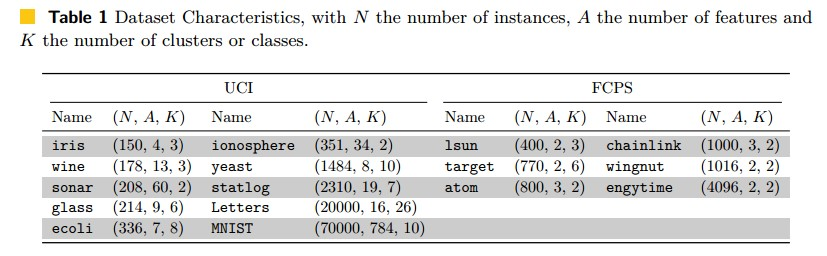
\includegraphics[width=0.5\linewidth]{./images/data.jpg}
        \caption{datasets}
    \end{figure}
\end{frame}

\begin{frame}{Parameters Setting}
    \begin{itemize}
        \item QUESTION:What effect do  $\alpha,\beta$ have on clustering results?
        \item $\alpha:\frac{\text{num}_\text{anchors}}{\text{size}_\text{cluster}}$
        \item $\beta:\frac{\text{num}_\text{super-instace}}{\text{size}_\text{cluster}}$
        \item dataset:all datasets
    \end{itemize}
    \begin{figure}
        \centering
        \subfigure[]{
            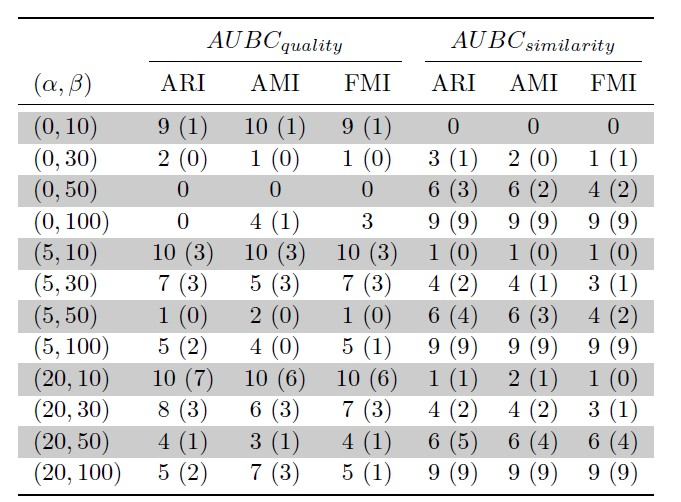
\includegraphics[width=0.4\linewidth]{./images/params.jpg}
        }
        \subfigure[use ARL]{
            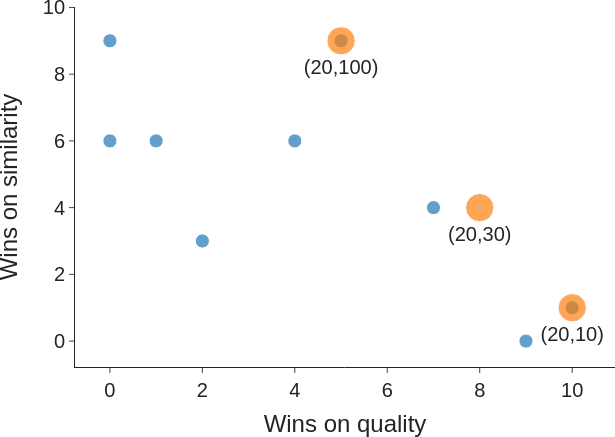
\includegraphics[width=0.4\linewidth]{./images/arl-params.png}
        }
    \end{figure}

    
\end{frame}



\begin{frame}{Runtime w.r.t Num\&Types of Constraints}
    \begin{itemize}
        \item randomly generate sets of four types of constraints
        \item initialize using KMeans
        \item average 90 runs
        \item Setting:$\alpha=0\%,\beta=100\%$
    \end{itemize}
    \begin{figure}
        \centering
        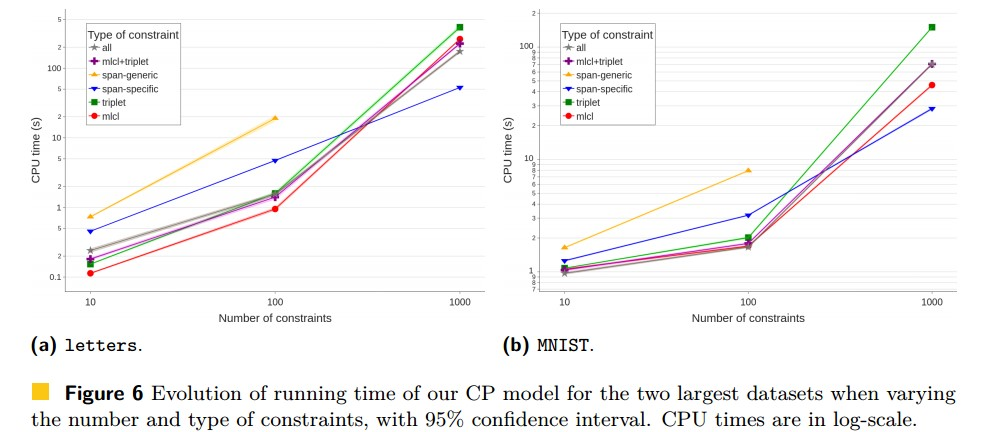
\includegraphics[width=0.8\linewidth]{./images/runtime-single.jpg}
    \end{figure}
    
\end{frame}

\begin{frame}{Comparison with Other Soft Constraint Methods}
    \begin{itemize}
        \item Q:IAC的relaxing constraint与其他方法的soft constraints相比如何?
        \item Setting:
        \begin{itemize}
            \item IAC+Anchors:$\alpha=20\%,\beta=100\%$,IAC+Anchors+Super-Instances:$\alpha=20\%,\beta=30\%$
            \item dataset:mk2
        \end{itemize}
    \end{itemize}
    \begin{figure}
        \centering
        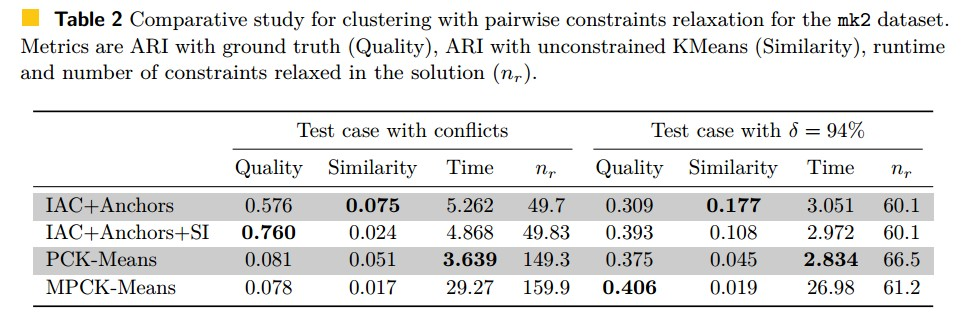
\includegraphics[width=0.8\linewidth]{./images/runtime-multi.jpg}
    \end{figure}

\end{frame}

\begin{frame}
    \frametitle{Comparison with Alternatives}
    \begin{itemize}
        \item $\alpha=20\%,\beta=30\%$
        \item 10 iterations of selection-modification loop
        \item glass dataset
    \end{itemize}
    
    \begin{figure}
        \centering
        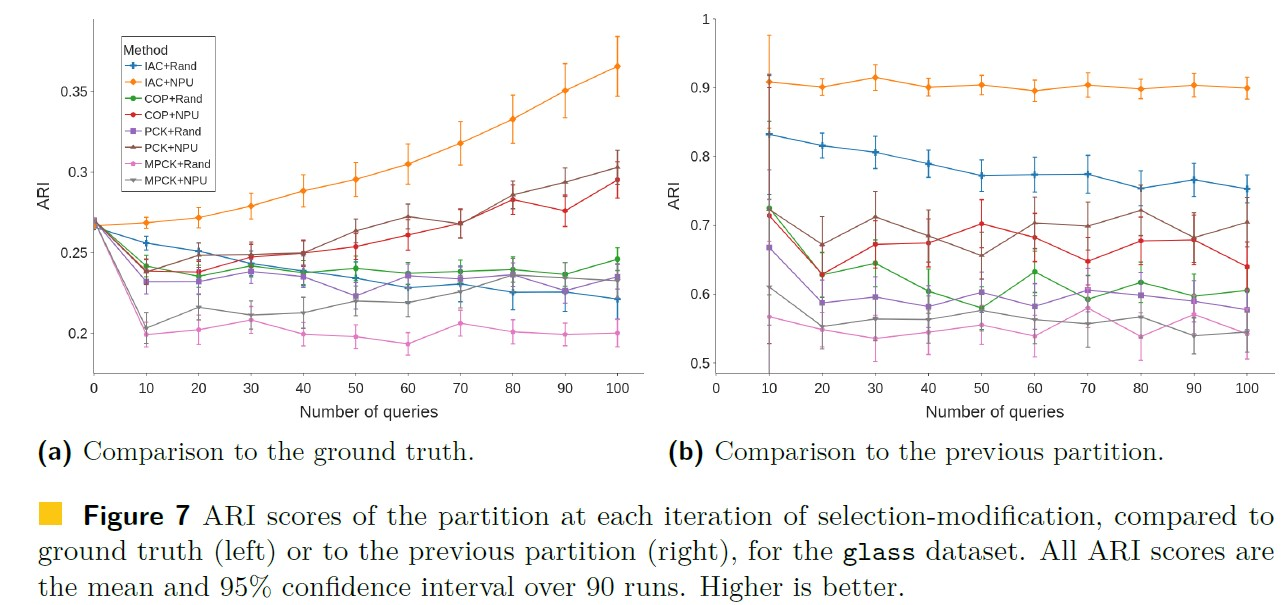
\includegraphics[width=0.8\linewidth]{./images/comp.jpg}
    \end{figure}
    \begin{itemize}
        \item more effective with NPU 
        \item IAC+NPU has the highest ARI
        \item IAC+NPU has the best similarity
    \end{itemize}
    

\end{frame}
\begin{frame}{Comparison with Alternatives}
    Modification time
    \begin{itemize}
        \item 虽然使用NPU能够使结果更好,但在较大数据(e.g. letters)上,耗时长,不适合用户交互。
    \end{itemize}
    
    \begin{figure}
        \centering
        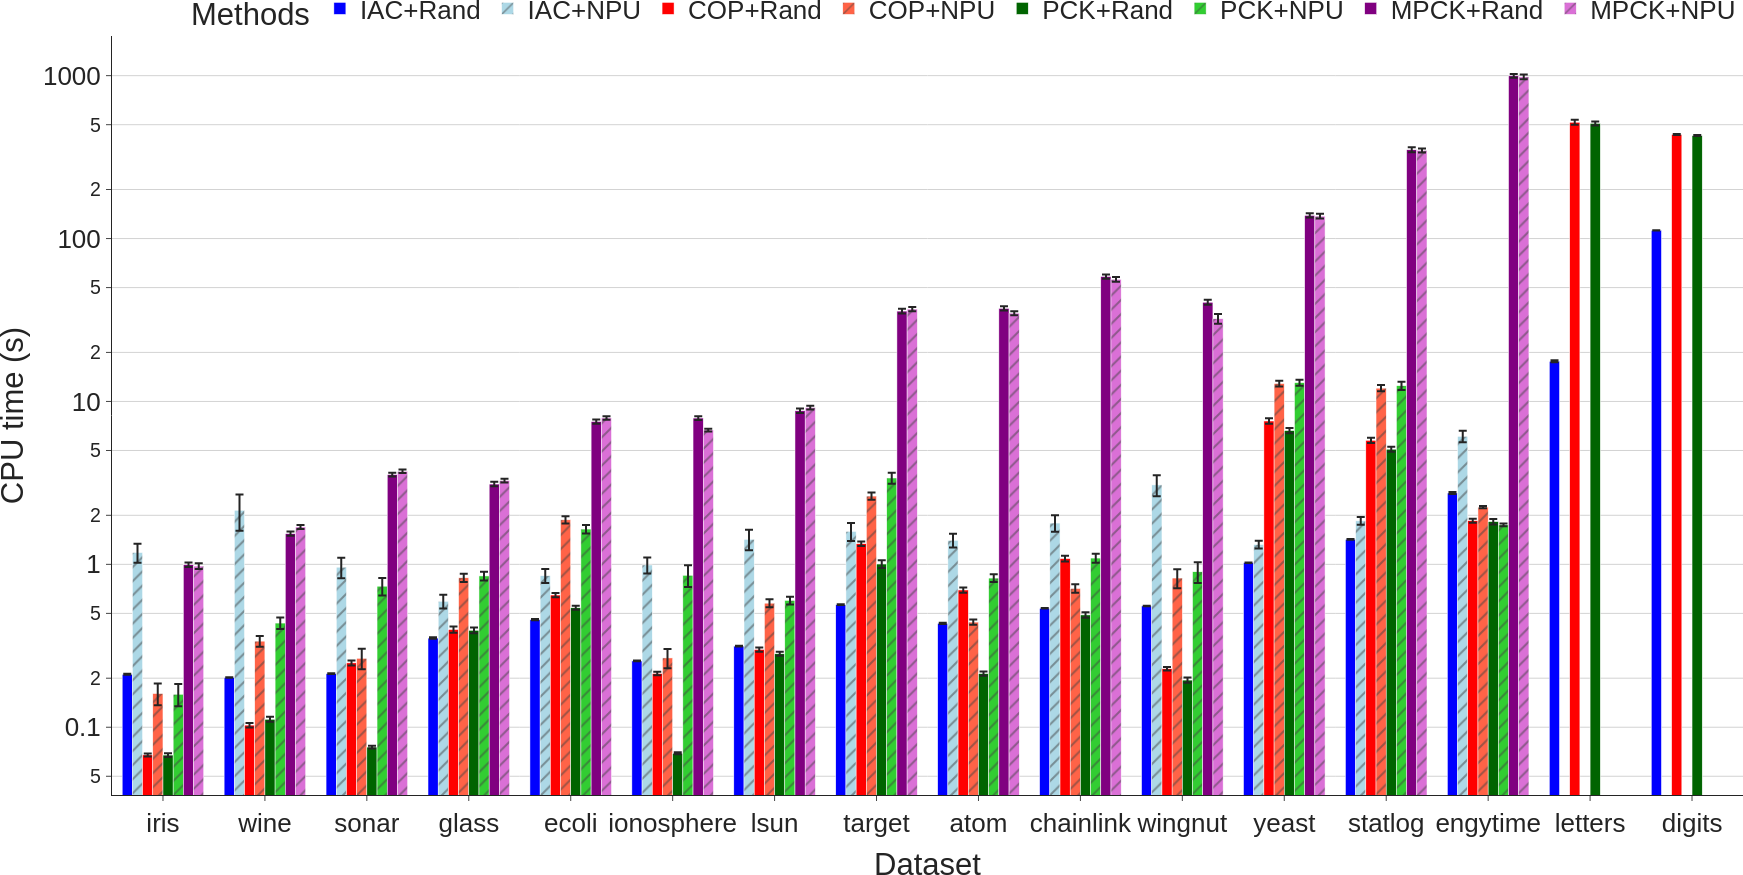
\includegraphics[width=0.8\linewidth]{./images/time.png}
    \end{figure}

    
\end{frame}

\begin{frame}{Tree Cut Data}
    \begin{itemize}
        \item Data:2016-2018年间11张724*337的山脉卫星图,每个像素都与一个NDVI(归一化植被指数)值相关联。
        \item classes:vegetation, artifficial structure, tree cut zones
        \item 特点:tree cut zones 被领域专家精确标记,但是占比只有不到0.3\%(637个点),难以被无监督方法发现。
        \item Problem Definition:根据专家提供的179个binary-constraints(图b),将tree cut zones(图a)发现出来。
    \end{itemize}
    \begin{figure}
        \centering
        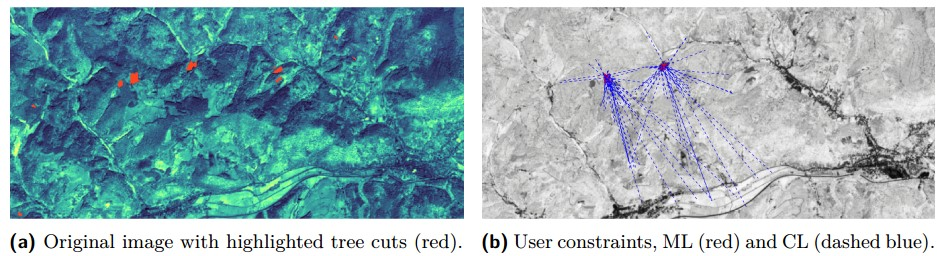
\includegraphics[width=0.8\linewidth]{./images/ab.jpg}
    \end{figure}
    
\end{frame}
\begin{frame}{Tree Cut Data}
    \begin{itemize}
        \item 设置:$\beta=1$,迭代至所有输入约束被满足
        \item 使用KMeans初始化15个簇,面积最大的簇作为positive cluster(图c着色部分),其他簇作为negative cluster(图c未着色部分)。将这种binary partition作为IAC输入。
        \item 结果为图b:
        \begin{itemize}
            \item green:true positive, yellor:false negetive, purple:false positive
            \item 两处主要的tree cut zone结果:左边TP从37/204$\rightarrow$94/204, 右边TP增加了10个。
        \end{itemize}
    \end{itemize}

    \begin{figure}
        \centering
        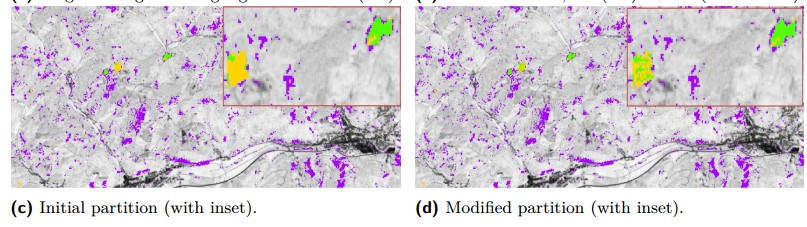
\includegraphics[width=0.8\linewidth]{./images/result.jpg}
    \end{figure}
\end{frame}
\section{conclusion}
\begin{frame}{conclusion}
    \begin{itemize}
        \item     提出了Incremental and Active Clustering Framwork(IAC),在Incremental setting中专家通过manually或active method来添加约束,从而使聚类有一定的连续性。
        \item IAC的运行时间依赖constraint selection这一步,需要更多的研究来提出适合incremental setting的active method。
        \item 如何重新利用relaxed constraints仍然是个open question。
    \end{itemize}


\end{frame}

\begin{frame}
    \begin{center}
        {\Huge\calligra Thanks!}
    \end{center}
\end{frame}

\end{document}